\documentclass[11pt]{amsart}
\usepackage{geometry}                % See geometry.pdf to learn the layout options. There are lots.
\geometry{letterpaper}                   % ... or a4paper or a5paper or ... 
%\geometry{landscape}                % Activate for for rotated page geometry
%\usepackage[parfill]{parskip}    % Activate to begin paragraphs with an empty line rather than an indent
\usepackage{graphicx}
\usepackage{amssymb}
\usepackage{epstopdf}
\usepackage{setspace} 
\usepackage{amsmath}
\usepackage{algorithm}
\usepackage{algpseudocode}
\usepackage{float}


\DeclareGraphicsRule{.tif}{png}{.png}{`convert #1 `dirname #1`/`basename #1 .tif`.png}

\title{Brief Article}
\author{The Author}
%\date{}                                           % Activate to display a given date or no date
\usepackage{parskip}
\setlength{\parindent}{18pt}

\begin{document}
\begin{spacing}{1.2}
\maketitle
%\section{}
%\subsection{}

\section{Report}

In the previous chapter, I have investigated techniques on different pre-processing strategies that can improve the performance of the general  DTW algorithm  in working with high dimensional time series datasets. These techniques that I am investigated so far primarily focus on the improving the quality of the data rather than the algorithm itself. The results found from the experiments so far, have shown that understanding the intrinsic properties of the data and factoring in the  domain information can not only improve the performance of the  DTW but may even discard the need for a  the  global windowing constraint(as we have seen for the model that augments feature selection and MFCC feature extraction) to reduce the time and computational complexity.  The DTW algorithm is a memory based algorithm that employs a similarity metric to compare a sequence with all sequences in the training in an iterative manner.  Since the whole training set is used during the testing phase, the computational complexity makes the algorithm very attractive to use. The computational cost of a DTW algorithm is $(mn)$ where $m$ and $n$ denote the length of the two time series sequences currently being compared. Using longer sequences increases the size of the DTW cost matrix hence resulting into a greater number of computations. The domain-dependent pre-processing methodology doesnt guarantee the dropping of the  global window constraint that is used to reduce the search space when tackling high dimensional data. As we have seen from the experiments,when working with high-dimensional time-series data, the accuracy of the DTW algorithm using a window constraint suffers greatly even if it's equipped with domain dependent/independent features. Hence from a scientific point of view, it is of great interest to research methods to improve the DTW algorithm so it can constraint the time and computational complexity associated with high-dimensional data without degrading the accuracy by too much. In this chapter, I investigate an unsupervised methodology that:


 %Time series sequences are embedded with local and global trends. Unsupervised methods using DTW  focus on  exploiting the information of either these trends for pattern extraction and mining. From the  work conducted by Xie and Wiltgen on  the time series datasets[], it  has been shown that using DTW equipped with features that incorporate  information of \textbf{both}  local trends and global shapes in the clustering /classification process greatly improve the performance of DTW . Unlike the MFCC, the features constructed from local and global trends are domain independent and thus can be applied to any time of data.  However, when working high-dimensional time-series data, the accuracy of the DTW algorithm using a window constraint suffers greatly even if it's equipped with domain dependent/independent features. Hence from a scientific point of view, it is of great interest to research methods to improve the DTW algorithm so it can constraint the time and computational complexity associated with high-dimensional data without degrading the accuracy by too much. In this chapter, I investigate an unsupervised methodology that:

\begin{itemize}
\item incorporates  information about local and global trends  in the feature extraction process
\item employs an adaptive DTW that tackles the issue of the large time and computational complexity by moving from working on  time series sequences to  sequences of segmented time-slices. To counter the tradeoff in the decrease  in accuracy, the algorithm is equipped with a kernel function(self-proposed) that is designed to measure the similarity of sub-sequences more accurately than standard euclidean metric by being invariant toward time-dilation and scale.   
\end{itemize}

\section {{Feature extraction}}


For feature extraction, the methodology that I have used  for this setup is based on Xie and Wiltgen's paper[] that I have already discussed in the previous section.  Each point in the time series sequence is replaced by a 4 dimensional vector  where the first two features correspond to information regarding the local trends around a point and the last two features reflect the position of that point in the global shape of the sequence.

Definition of local feature as  given in [] :
\[ f_{\mbox{local}}(r_i)= (r_i-r_{i-1}, r_i-r_{i+1})\]

Definition of global feature:
\[ f_{\mbox{global}}(r_i)= (r_i -\sum_{k=1}^{i-1}\frac{r_k}{i-1} , r_i-\sum_{k=i+1}^M \frac{r_k}{M-i})\]


\section{Adaption of DTW}
The feature extraction methodology discussed above maps the time series sequence to a time series sequence of vectors whose length  is $\|X_n\|-2. $   ( where $\|X_n\| $ denotes the  length of the original time series sequence).  The DTW augmented with these features will still suffer from large time and computational complexity if the dimensionality of the data is high. In the MFCC feature extraction process, the time series sequence is first segmented into series of frames  of length 20ms. Through appropriate functional mapping, each  frame is then mapped to a vector. Because the length of the resultant sequence of vectors is much smaller than the length of the original time series, the size of the  DTW cost matrix is reduced resulting in lower  time and computational cost associated with each comparison.

Similar to the MFCC extraction process, the time series of 4d vectors extracted in the feature extraction stage are segmented using windows  of width 5ms. The original time series is reduced to series of matrices  where the length of the new  series is 5 times smaller than before. Now if we adapt the cost function of DTW to work on series of matrices rather than series of vectors we can achieve a large improvement in the time and computational cost  associated in the testing phase without imposing a \textbf{window} constraint. 

The problem now can be shifted to finding  an appropriate kernel that can be used to compute the similarity between matrices composed of feature vectors. Ideally, we want a metric that takes into account the variation of speed and time when comparing two similar subsequences. We will want to compare the global and local properties associated with a point in one subsequence with the global and local properties of points at  different regions in the second sub-sequence illustrated by figure 2.  Using a euclidean metric in this scenario is inappropriate. The euclidean metric  in this context is identical to  linear time warping where the  two subsequences will be matched based on a linear match of the two temporal dimensions.  In our context, we need a kernel that computes the similarity between two sub-sequences by warping the time axis.

The motivation behind the kernel  that I propose for aiding  DTW to tackle  high-dimensional data comes from the polynomial kernel. \\
Let $x$ and $z$ be two dimensional vectors.
Consider the simple polynomial kernel of degree 2  :$k(x,z) = (x^{T}z)^2$ .  This kernel can expressed as :
\begin{eqnarray*}
k(x,z) &= &(x^{T}x')^2\\
&  =& (x_1z_1+x_2z_2)^2\\
&= & x_1^2z_1^2 + 2x_1z_1x_2z_2 + x_2^2z_2^2\\ 
&=& (x_1^2, �2x_1x_2, x_2^2)(z_1^2, �2z_1z_2, z_2^2)^{T}\\
&=& \phi(x)^{T}\phi(z)\\
\end{eqnarray*}\\
The 2nd order polynomial kernel is equivalent to a corresponding feature mapping $\phi$  that contains terms of order 2. Now, if we generalise this notion then $k(x,z) = (x^{T}z)^M$ contains all monomials of order M. If we imagine x and z to be two images, then the polynomial kernel represents a particular weighted sum of all possible products of M pixels in the first image with M pixels in the second image.\\
Using this as motivation I propose the following kernel:.
\[ k(x,z) = <\sum_{i=1}^{n}x_i, \sum_{j=1}^{n}z_j>\]
where $n$ denotes the length of the window and $x_i$  and $z_j$ represents the 4-dimensional features indexed by the points in two sub-sequences.\\
To motivate the reasoning behind the construction of this particular kernel lets consider the following signals:
\begin{figure}[H]
  \centering
   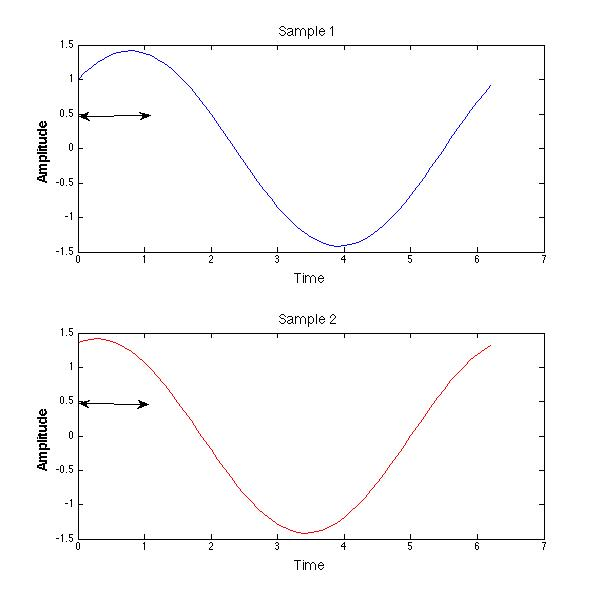
\includegraphics[scale=0.4]{Example1.jpg}
  \caption{Two signals separated by translation}
 \end{figure}
The signal denoted by the `red' color is a `slower' version of the signal denoted by the `blue' color . In the above example, if we are comparing the similarity  between the  time slices spanned by the arrows, an ideal kernel must be invariant to  the time offsets of the signals and thus should consider all possible pairings between the vectors in the subsequences. Intuitively speaking, the kernel must behave like a DTW algorithm..\\
\begin{figure}[h!]
  \centering
   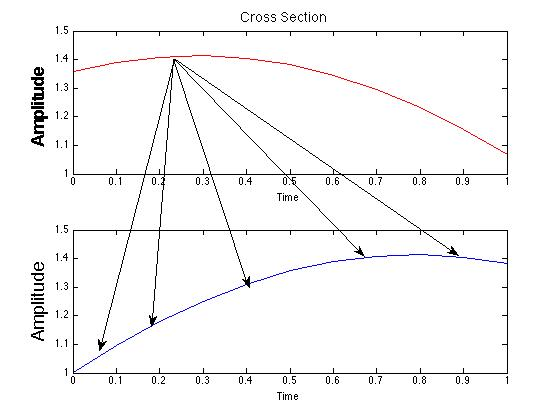
\includegraphics[scale=0.6]{Cross-section.jpg}
  \caption{Two identical subsequences varying in time }
  \end{figure}
 For time slices of width $n$, the kernel  metric  can be expanded and   expressed as :
\begin{eqnarray*}
k(x,z) &= &<\sum_{i=1}^{n}x_i, \sum_{j=1}^{n}z_i>\\
&  =& <(x_1+x_2+x_3+..),(z_1+z_2+z_3+..)>\\
&= & <x_1,z_1>+<x_1,z_2>+<x_1,z_2>...+<x_2,z_1>+<x_2,z_2> +<x_2,z_3>+......\\ 
\end{eqnarray*}
From above expression, we can see  that the proposed kernel corresponds to a sum of all possible dot products of pairs belonging to the set
$\{(x_iz_i) | x_i\in \mbox{seq1}, z_i \in \mbox{seq2}\}$. Similar to the polynomial kernel, the proposed kernel  allows us to match all possible pairs of vectors belonging to the two sub-sequences  given by the matrices.
It is easy to check that this proposed kernel is in fact a valid kernel:
\begin{itemize} \itemsep-2pt
\item K(x,z)= K(z,x) $\Rightarrow $the function is symmetric.
\item The kernel satisfies Mercer's theorem : K(x,z) =$\phi(x)^T\phi(x)$
where  the feature mapping corresponds to  a finite summation of vectors $\phi(y) = \sum_{i=1}^{n}y_i$. 
\end{itemize}
Augmenting the kernel to the DTW algorithm allows DTW to work on high-dimensional time sequences with using a window constraint. However the accuracy and computational cost of the DTW is now dependent on the size of the time slices used to segment the original sequences:
\begin{itemize} \itemsep-2pt
\item The accuracy of DTW increases as the width of the windows decrease. Using subsequence allows the similarity measure to be dominated by the dot products of points whose local and global features are most alike. However using smaller windows achieve lesser dimensionality reduction. Thus the time and computational complexity suffers.
\end{itemize}
To use this kernel as an  appropriate cost function in the DTW algorithm, we need a functional mapping that:
\begin{enumerate} \itemsep-2pt
\item  constraints the codomain to be in the range from 0 to $\infty$.
\item    ensures larger values given by the function signify great degree of dissimilarity and smaller values  signify a high degree of similitude.
\end{enumerate}
An ideal cost function that make use of dot product sis the \emph{arc-cosine}. Hence I embedded the kernel function in the cosine distance: 
\[ \theta = \frac{ <X,Z>}{|X||Z|} \]
where $X = \sum_{i=1}^{n}x_i$ and $Z =\sum_{j=1}^{n}z_i$

A formal outline of the algorithm is as follows:

 \begin{algorithm}
\begin{algorithmic}[1]
\Procedure{Value-based}{$seq1,seq2$}\Comment{two sequences of feature vectors}
\State  seq\_1$\leftarrow$segment(seq1,n)\Comment{ Segment the sequences using a window of size n}
 \State seq\_2$\leftarrow$segment(seq2,n)
 \For{i=1: to length(seq\_1) } \Comment{Initialise the DTW cost matrix}
 \State DTW(i,0) = $\infty$
 \EndFor
 
 \For{i=1 to length(seq\_2)}
 \State DTW(0,i) = $\infty$
 \EndFor
  \For{i=2 to length(seq\_1)}  
 \For{j=max(2, i-w) to min(length(seq\_2), i+w)} 
 
  \State DTW(i,j) = $\theta = \frac{ <X,Z>}{|X||Z|} $+ min\{ DTW(i-1,j)+DTW(i,j-1)+DTW(i-1,j-1)\}
 \EndFor \Comment { $X = \sum_{i=1}^{n}x_i$ and $Z =\sum_{j=1}^{n}z_i$}

 
 \EndFor
\State \texbf{return}  result = $\frac{\mbox{DTW(n,m))}}{nm}$ \Comment{n=length(seq1), m=length(seq2)}

\EndProcedure
\end{algorithmic}
\caption{Adpated DTW}
\end{algorithm}
 

\newpage

\section{Experimental results}
The changes that I have introduced,  in the previous section  to the `Dynamic Time Warping' algorithm is aimed to improve the algorithm's performance in handling high dimensional time series data. In this section, I investigate the investigate the performance of my proposed algorithm by running it  on the test data set that I have constructed from TIDIGITS test corpus and the time complexities and accuracies  against the methodologies that I have investigated so far:
 
\begin{itemize}
\item Approach 1
\begin{itemize}
\item Apply feature selection process to remove segments of silence and down sample the remaining segment to improve the quality.
\item  Apply value-based DTW(which we denote as baseline) using the most constrained window size  and a euclidean metric.
\end{itemize}

\item Approach 2
\begin{itemize}
 \item Apply no feature selection process
 \item Perform feature extraction by extracting MFCC features
 \item Apply DTW using the most constrained window size and a euclidean metric.
 \end{itemize}
 
 \item  Approach 3
 \begin{itemize}
 \item Apply feature selection process that only removes  segments of  silence 
 \item Extract MFCC features
 \item Apply DTW augmented with the euclidean metric.
 \end{itemize}

 
\item Approach 4
\begin{itemize}
\item Apply feature selection process to remove segment of utterance and down sample the remaining segment to improve the quality.
\item Apply  the feature extraction process discussed in [] to extract local and global features.
 \item Apply DTW using the most constrained window size  and a euclidean metric.
 \end{itemize}


 
 
 \end{itemize}


\begin{figure}[h!]
  \centering
   
     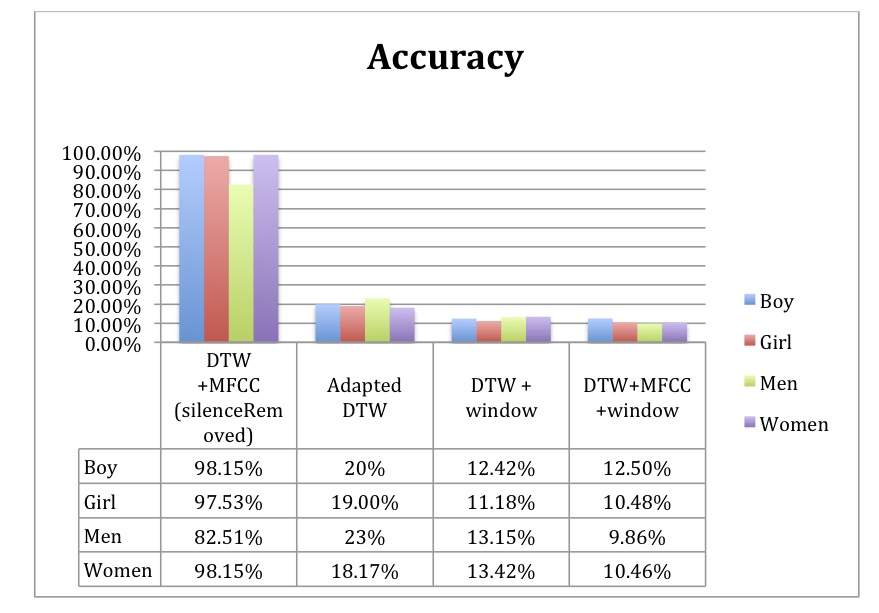
\includegraphics[scale=0.8]{Accuracy.jpg}
  \caption{Accuracy}
  
\end{figure}
\end{spacing}
\begin{figure}[H]
  \centering
   
   
     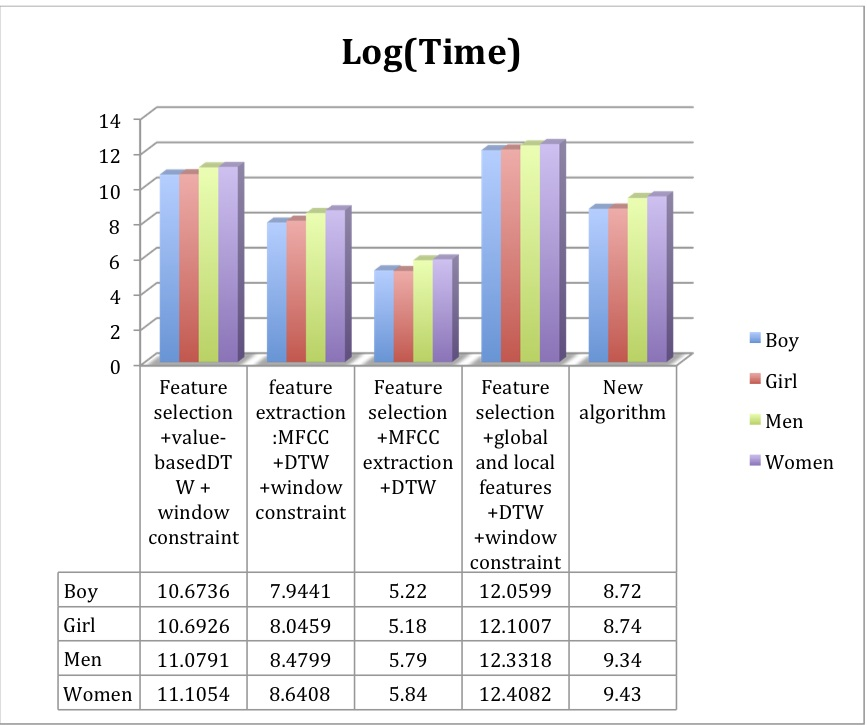
\includegraphics[scale=0.8]{GraphsResults.jpg}
  \caption{Time complexity}
  \end{figure}

There are quite number of interesting observations that can made from the graphs and the tables given by figures []. 

\begin{itemize}
\item The proposed algorithm achieves better accuracy for test samples belonging to all categories than any of algorithms that employ the rigid  window constraint of  $w = max(\lceil{0.1*max(n.m)}\rceil, abs(n-m))$. The most interesting result is that the new algorithm incurs a lower computational cost than any of these DTW algorithms. 
\item From examining the improvements in accuracy across all categories, it can be concluded that for the TIGITS dataset,  the new algorithm is invariant to variations introduced  in the acoustic signals  by different speakers . 
\item The  methodology behind my proposed approach and that of  approach 4  includes the same pre-processing stage. Th input to the DTW algorithm is constructed by using  the domain dependent feature selection process mentioned in section followed by a domain independent feature extraction mapping (i.e the local and global features defined in section).  Both approaches  differ however, in their use of a cost function and a window constraint. The proposed approach doesn't subject DTW  to any window constraints and utilised the kernel function that I constructed in the cost metric. Approach 4 on the other hand, employs the euclidean metric an subjects DTW to the window constraint of  of $w = \mbox{max} (|n-m|,\ceil{0.1*\mbox{max}(n,m))$.

The proposed DTW segments sequences into frames and employ a cost function on  the frames. This reduces the dimensionality of the time series sequences and allows the algorithm to achieve a  time and computational cost than is lower than  the cost incurred by any of the investigated adaptations of the DTW algorithm that  employs window constraints. 
\end{itemize}

  To confirm that the performance of the new algorithm  is not tailored for this particular time-series data set, I have applied the tested the algorithm on the two largest  time series data sets in UCR database. 
  
  The description of the data sets used for the next set of experiements are as follows:
  \begin{enumerate}
  \item CinC\_ECG\_torso
  
  \begin{itemize}
    \item Length of the time series:1639
  \item Size of test set:1380
  \item Size of training set:40
  \item Number of classes:4
  \end{itemize}
  \item  InLineSkate
  \begin{itemize}
    \item Length of the time series:1882
  \item Size of test set:550
  \item Size of training set:100
  \item Number of classes:7 
  \end{itemize}
  
  Unlike the speech utterances, the time series sequences within each data set  share the same length.
  
  \subsection{Experimental setup}
  
 The focus now is  to check how well/ bad is the performance of the new DTW algorithm  against  DTW algorithms using window constraints when applied to datasets that belong to other application domains . The domain -dependent pre-processing policies are dropped for this set of experiments as these procedures were specifically designed for speech data. Thus in this section, I compare my proposed approach against:
 \begin{itemize}
 \item Approach 1
 \item Approach 4 
 \end{itemize}
  As a I mentioned, the domain-dependent feature selection process  of silence removal and subsampling is dropped from all approaches. However, the feature extraction process  that involves extracting  local and global features is kept since this procedure is domain independent.
  
One of the factors that I have also investigated in these experiments is  the size of the time slices used in the algorithm that I proposed. For the TIDIGITS data set, I have used window slices of 50 ms. Reducing the size of the windows should principally increase both accuracy and time-complexity .
The core kernel used by the new algorithm is based on the function: 
\[ k(x,z) = <\sum_{i=1}^{n}x_i, \sum_{j=1}^{n}z_j>\]
k(x,z) represents the sum of all possible dot-products . Having a smaller window allows the sum to be dominated by dot products of vectors that are most similar. However smaller window  frames results in  longer time series sequence of frames. This in turn increases the time and computational complexity incurred by the DTW algorithm.
  
Figure [] and figure[] shows the  accuracies and log(time) of the  algorithms  for the two datasets:

  \begin{figure}[H]
  \centering
   
     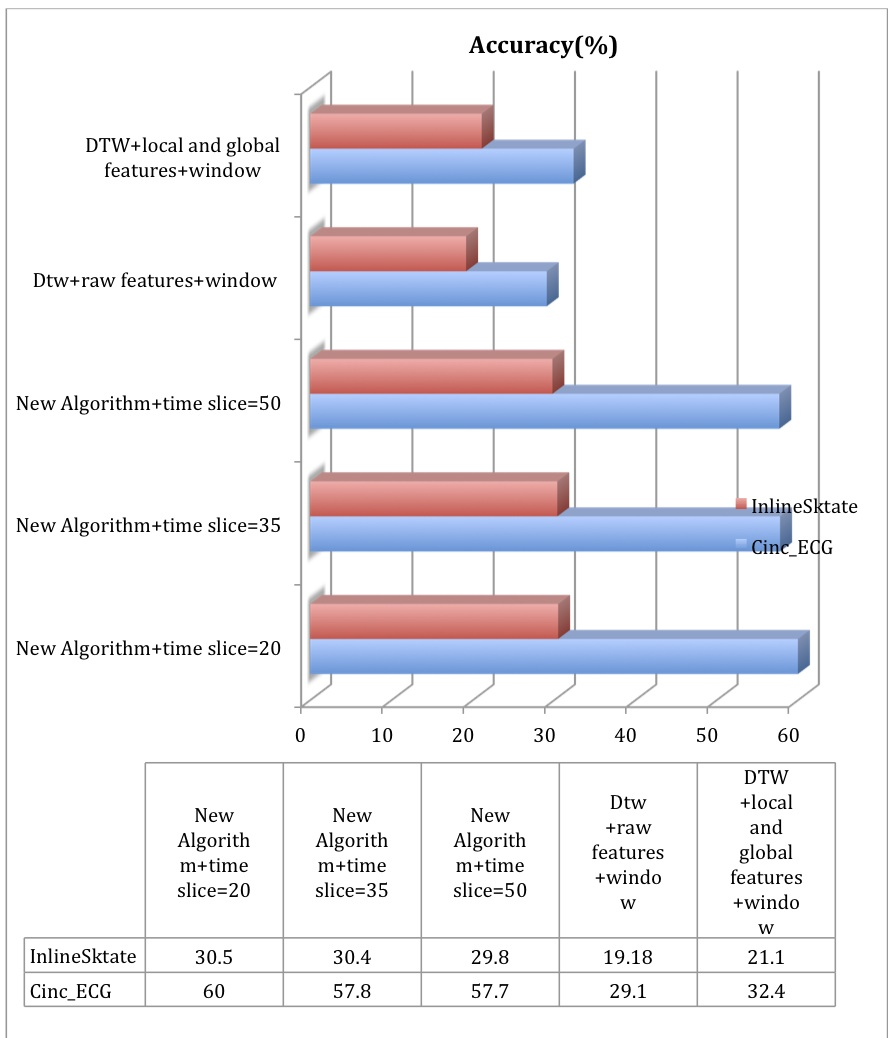
\includegraphics[scale=0.8]{accuracy_cinc_inline.jpg}
  \caption{Accuracy}
  \end{figure}
   
   Observation:
   \begin{itemize}
   \item The  new algorithm indeed achieves better accuracy than any versions of the window  constrained DTW algorithm employing domain-independent feature extraction
   \item Comparatively, the performance of the new algorithm does improve if smaller window slices are employed to partition the time series sequence of vectors. 
   \end{itemize}
   
   
\begin{figure}[H]
  \centering
   
     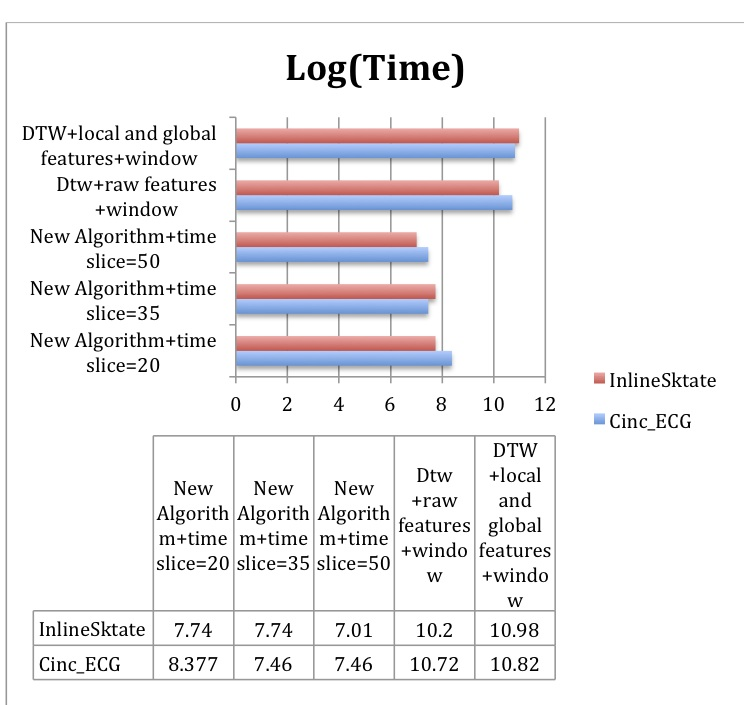
\includegraphics[scale=0.8]{time_cinc_inline.jpg}
  \caption{Time complexity}
  \end{figure}
Observation:
   \begin{itemize}
   \item The  new algorithm incurs less time and computational cost  than any versions of the window  constrained DTW algorithm employing domain-independent feature extraction
   \item Comparatively, the time complexity of the new algorithm increases when smaller window slices are used to partition the sequence
   \end{itemize}   

\end{spacing}

\end{document}  